\section{Introduction}

Descriptions of LLM agents use inconsistent terminology for the software around the model: \emph{framework}, \emph{scaffold}, \emph{runtime}, \emph{orchestration layer} and \emph{harness} are all in common use. When the underlying systems are examined, however, they share a common mechanism:

\begin{enumerate}
\def\labelenumi{\arabic{enumi}.}
\tightlist
\item
  a model is called;
\item
  some component determines what the call contains;
\item
  some component acts on what the call returns;
\item
  some component decides whether to call again.
\end{enumerate}

The terminology varies; the mechanism does not.

The absence of a shared decomposition has practical costs.

\begin{itemize}
\tightlist
\item
  \textbf{Diagnosis.} Without names for an agent's parts, a failure cannot be attributed to a part.
\item
  \textbf{Comparison.} Systems described in different terms cannot be compared directly.
\item
  \textbf{The product landscape.} The same few ideas recur as separate products: memory layers, model gateways, tool protocols, tracing platforms, sandboxes and evaluation suites. Without a map, it is unclear which of them are new and which are existing ideas under new names.
\end{itemize}

Recent work establishes that this layer matters. Zhang et al.~\cite{zhang2026stop} argue that, among comparable frontier models, harness configuration can account for more of the variance in performance than the choice of model, and that agents should therefore not be compared without disclosing their harnesses. Fan et al.~\cite{fan2026empirical} hold a coding harness's loop fixed and vary three of its parts (planning, the action space and context management), finding that each alters agent behavior. Both treat the harness as a primary determinant of agent behavior. Fan et al.~select parts of a harness to vary; the present work asks what the complete set of parts is.

Our approach is \textbf{reductive}: we decompose an agent until its parts are no longer shared across systems. It is also \textbf{mechanistic}: each part is defined by its function on the path from request to response, not by its name or by the product that provides it.

\textbf{Contributions.} Contributions 1--3 constitute the core of the paper; contributions 4--6 follow from them.

\begin{enumerate}
\def\labelenumi{\arabic{enumi}.}
\tightlist
\item
  \textbf{A two-component view of agents,} Agent = Harness(Model), in which the model is a fixed function and all else is harness (§2).
\item
  \textbf{Five primitives of a harness,} each with a positive and a negative definition, together with rules for resolving cases at their boundaries (§3--4).
\item
  \textbf{A constructive argument for sufficiency:} a working agent built one primitive at a time, in which each step's deficiency is the next primitive (§5).
\item
  \textbf{A reduction of production concerns} to hardening within the primitives (§6).
\item
  \textbf{A decomposition of three production harnesses,} Claude Code, Codex and opencode, which finds no need for a sixth primitive and refines the boundary rules (§7).
\item
  \textbf{A case study} in which the constructed agent produced much of its own teaching material (§8).
\end{enumerate}

This is a conceptual and analytical contribution, in the tradition of frameworks such as CoALA \cite{sumers2024cognitive}: its evidence is a construction, a decomposition of existing systems, and a case study, and it reports no quantitative experiments. Measuring how much each primitive contributes to differences in performance is left to future work (§9.5).

The paper is accompanied by a companion artifact, \emph{harness-engineering} \cite{course}, an open course with runnable code. The artifact builds the harness of §5 and the production layers of §6 incrementally and retains full transcripts of every run. The paper is self-contained: every listing and run on which the argument depends is reproduced in Appendices A--D.

\section{Two components: the model and the harness}

\subsection{The model}

The model predicts. Given a sequence of tokens, it produces a distribution over the next token:

\begin{quote}
\textbf{TokensOut = Model(TokensIn)}
\end{quote}

Viewed from outside, the model is a function. It retains no state between calls, cannot read from or act on its environment, and cannot initiate a further call. Everything it knows about the present moment is contained in its input. The model is the product of \emph{model development} (training data, compute, and methods for training and evaluation), a separate discipline whose output we treat as fixed.

\subsection{The harness}

The harness comprises everything else. It determines how inputs are gathered, how they are presented to the model, how the model is called, how its outputs are handled, and how information flows among these steps:

\begin{quote}
\textbf{Agent = Harness(Model)}
\end{quote}

\emph{Harness engineering} is the construction of this second component.

The division is deliberately coarse. Anything that is not the model's weights is harness: a system prompt, a tool, a retry policy, a memory store. Two agents built on the same model differ only in their harnesses; a comparison that omits the harness therefore omits the variable under study.

\subsection{Method}

The decomposition proceeds by repeated application of a single question:

\begin{quote}
\emph{What is it, and by what mechanistic primitives does it work?}
\end{quote}

Applied to an agent, the question yields a model and a harness. Applied to a harness, it yields five primitives (§3). Applied once more, to a primitive, it yields answers that are no longer shared across systems: one harness's input reads a terminal, another's a chat channel, a third's a webhook. We take this as the stopping criterion. A primitive is the deepest level at which every harness still has the same parts.

Each primitive is given two definitions:

\begin{itemize}
\tightlist
\item
  a \textbf{positive} definition, stating what it does;
\item
  a \textbf{negative} definition, stating what it never does and naming the primitive responsible for that function instead.
\end{itemize}

The negative definitions carry most of the analytical weight. They make the primitives mutually exclusive, so that each piece of harness code has exactly one home. A piece is assigned by \textbf{its function, not by its location in the code} or by its name (§4).

\subsection{Scope}

The primitives describe what happens on the path of a request at run time. Some software that ships with a harness never acts on that path, and we exclude it, as we exclude model development:

\begin{itemize}
\tightlist
\item
  \textbf{transport and hosting:} client/server splits, remote workspaces, the process serving a user interface;
\item
  \textbf{persistence:} databases;
\item
  \textbf{event wiring:} internal event buses;
\item
  \textbf{configuration and packaging:} settings loaders, plugin installers.
\end{itemize}

These components carry, store or configure the primitives without constituting a step in a pass. Where such a component does act on the path, for example a saved transcript that the harness replays, that action is assigned like any other.

\section{The five primitives}

\begin{figure}[t]
\centering
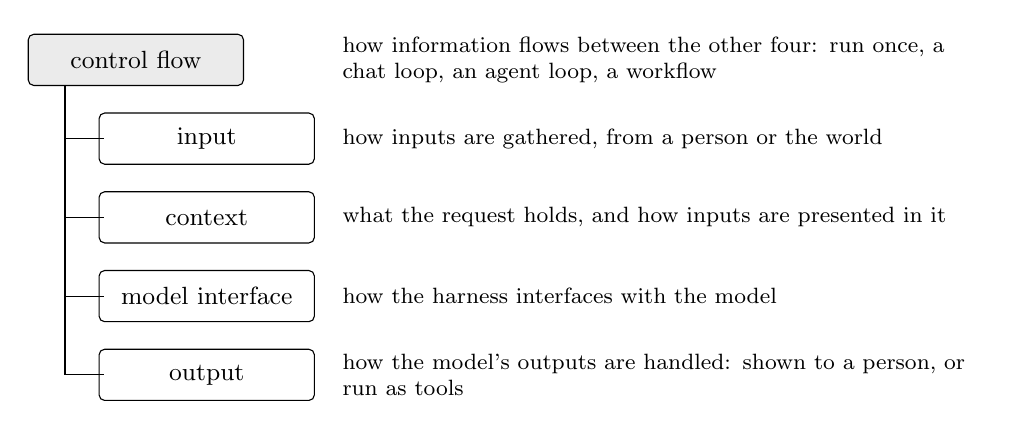
\begin{tikzpicture}[
  box/.style={draw, rounded corners=2pt, minimum height=6.5mm, text width=25mm, align=center, font=\small},
  note/.style={font=\footnotesize, text width=80mm, align=left, anchor=west}]
\node[box, fill=black!8] (cf) at (0,0) {control flow};
\node[note] at (2.5,0) {how information flows between the other four: run once, a chat loop, an agent loop, a workflow};
\foreach \y/\name/\txt in {-1/input/{how inputs are gathered, from a person or the world},
                           -2/context/{what the request holds, and how inputs are presented in it},
                           -3/model interface/{how the harness interfaces with the model},
                           -4/output/{how the model's outputs are handled: shown to a person, or run as tools}} {
  \node[box] at (0.9,\y) {\name};
  \node[note] at (2.5,\y) {\txt};
  \draw (-0.9,\y) -- (-0.4,\y);
}
\draw (-0.9,-0.33) -- (-0.9,-4);
\end{tikzpicture}
\caption{The five primitives of a harness. Control flow wraps the other four.}
\label{fig:tree}
\end{figure}


One pass through a harness follows a single path:

\begin{figure}[t]
\centering
\begin{tikzpicture}[
  node distance=3.5mm,
  prim/.style={draw, rounded corners=2pt, minimum height=8mm, align=center, font=\footnotesize, fill=black!6},
  data/.style={font=\footnotesize\itshape, align=center},
  >=Latex]
\node[data] (pw) {person\\or world};
\node[prim, right=of pw] (in) {input};
\node[prim, right=of in] (ctx) {context};
\node[data, right=of ctx] (req) {request};
\node[prim, right=of req] (mi) {model\\interface};
\node[data, right=of mi] (resp) {response};
\node[prim, right=of resp] (out) {output};
\node[data, right=of out] (pw2) {person\\or world};
\draw[->] (pw) -- (in); \draw[->] (in) -- (ctx); \draw[->] (ctx) -- (req);
\draw[->] (req) -- (mi); \draw[->] (mi) -- (resp); \draw[->] (resp) -- (out); \draw[->] (out) -- (pw2);
\draw[->] (out.south) -- ++(0,-6mm) -| node[pos=0.25, below, font=\footnotesize\itshape] {result} (in.south);
\end{tikzpicture}
\caption{One pass through a harness. A tool's result comes back as input; control flow decides whether to go around again.}
\label{fig:path}
\end{figure}


Input gathers what is to be sent. Context assembles it into a request and fits it to the model's window. The model interface sends the request and receives the response. Output handles the response, either presenting it to a person or executing a tool; a tool's result re-enters as input. Control flow determines what happens at the end of the path: another iteration, a turn for a person, or termination.

\subsection{Model interface}

\textbf{Does:} sends tokens to the model as a request and receives tokens as a response.

\textbf{Never does:} decide when to call (control flow), gather what is sent (input), determine how it is presented (context), or act on what is returned (output).

The model interface is the thinnest primitive, as a consequence of its position. The other four operate on the harness side; the model interface is the boundary itself, the parentheses in \emph{Agent = Harness(Model)}. Its minimal form is a single SDK call. Richer implementations vary along several dimensions: the destination of the request (a hosted API, a local model, a gateway); its transport (an SDK, raw HTTP, a cross-provider translation layer); which model responds (a single model, or a backup when the first is unavailable); how the response arrives (whole or streamed); how many requests are sent (singly or in batches); failure handling (retries, backoff, timeouts); and request settings (output limits, reasoning effort, thinking summaries). All of these concern the delivery of one request and the receipt of one response.

\subsection{Input}

\textbf{Does:} gathers what is sent to the model, from a \textbf{person} (a task, a question, a message) or from \textbf{the environment} (the result of a tool execution: its output, its exit status, whether it failed).

\textbf{Never does:} determine how what it gathers is laid out in the request (context), send it (model interface), or decide whether to iterate (control flow).

Input is the harness's afferent pathway. Its sources include command-line arguments, prompts, pipes, chat applications, webhooks and schedules; its content may be text, images or files. Whatever the source, its function is to bring something from outside the harness to the edge of the request.

\subsection{Output}

\textbf{Does:} handles the model's response, either by \textbf{presenting} it to a person or by \textbf{executing} it as a tool call.

\textbf{Never does:} decide whether a tool's result is returned to the model (control flow), or determine what the next request contains (context).

Output is the efferent pathway. The model cannot act, but it can request an action: its response may contain a tool call, consisting of a name and arguments in a schema the harness has described to it. Output executes the call, and the result returns as input. The model requests; the harness acts. The design choices within output include which tools exist (one general tool or many specific ones); where they execute (locally, in a container, on a remote host, or at the provider); whether multiple calls execute sequentially or concurrently; when not to execute (a call truncated mid-generation is incomplete, and executing a partial command is worse than executing none); and how failures and hangs are handled.

Input and output are constructed independently but form two ends of a single exchange, which meets at the tool: output executes the call and input returns its result.

\subsection{Control flow}

\textbf{Does:} \textbf{sequences} the other four primitives, passing each one's product to the next, and \textbf{terminates}, deciding when to stop or return control to a person.

\textbf{Never does:} send the request (model interface), gather (input), present (context), or handle the response (output).

Control flow is the only primitive that contains the others. Its arrangement of them determines the kind of system that results.

{\def\LTcaptype{none} 
\begin{longtable}[]{@{}
  >{\raggedright\arraybackslash}p{(\linewidth - 4\tabcolsep) * \real{0.3333}}
  >{\raggedright\arraybackslash}p{(\linewidth - 4\tabcolsep) * \real{0.3333}}
  >{\raggedright\arraybackslash}p{(\linewidth - 4\tabcolsep) * \real{0.3333}}@{}}
\toprule\noalign{}
\begin{minipage}[b]{\linewidth}\raggedright
Shape
\end{minipage} & \begin{minipage}[b]{\linewidth}\raggedright
Arrangement
\end{minipage} & \begin{minipage}[b]{\linewidth}\raggedright
Who determines the next step
\end{minipage} \\
\midrule\noalign{}
\endhead
\bottomrule\noalign{}
\endlastfoot
Single call & input \(\rightarrow\) call \(\rightarrow\) output, then stop & no one; it is fixed \\
Chat loop & call, present, return to the person, repeat & the person \\
Workflow & the harness code fixes the sequence of calls (e.g., draft, evaluate, revise) & the harness code \\
Agent loop & call; while the model requests tools, execute them, return the results, call again & the model \\
\end{longtable}
}

The distinction between a \emph{workflow} and an \emph{agent} \cite{schluntz2024building} is thus a property of control flow: which party determines the next step. Termination is an equal half of the definition. A loop without a defined termination condition has no bound on its cost. The minimal agent loop terminates when the model stops requesting tools; richer implementations also terminate on step limits, spending limits, refusals, or a person's instruction.

\subsection{Context}

\textbf{Does:} before every call, \textbf{assembles} what the request contains and \textbf{fits} it to the model's context window.

\textbf{Never does:} gather inputs (input), send the request (model interface), or decide when to call (control flow).

Each call begins without state. The model has no knowledge of its environment, the date, its own identity, its previous actions, or earlier instructions unless the harness includes them in the request. For this reason, a large share of what is built into harnesses is context. The following components are all means of determining what the model sees:

\begin{itemize}
\tightlist
\item
  \textbf{instructions:} the system prompt;
\item
  \textbf{working memory:} the current session;
\item
  \textbf{episodic memory:} prior sessions;
\item
  \textbf{semantic memory:} durable facts;
\item
  \textbf{procedural memory:} skills, recipes and playbooks;
\item
  \textbf{retrieval:} search results inserted into the request;
\item
  \textbf{compaction:} a summary substituted for history that no longer fits;
\item
  \textbf{self-knowledge:} the agent's own description or source.
\end{itemize}

Input and context are distinct. Input brings an item to the edge of the request; context determines whether it is included, where, in what form, and what is removed to accommodate it.

\subsection{Summary}

{\def\LTcaptype{none} 
\begin{longtable}[]{@{}
  >{\raggedright\arraybackslash}p{(\linewidth - 4\tabcolsep) * \real{0.3333}}
  >{\raggedright\arraybackslash}p{(\linewidth - 4\tabcolsep) * \real{0.3333}}
  >{\raggedright\arraybackslash}p{(\linewidth - 4\tabcolsep) * \real{0.3333}}@{}}
\toprule\noalign{}
\begin{minipage}[b]{\linewidth}\raggedright
Primitive
\end{minipage} & \begin{minipage}[b]{\linewidth}\raggedright
Does
\end{minipage} & \begin{minipage}[b]{\linewidth}\raggedright
Never does
\end{minipage} \\
\midrule\noalign{}
\endhead
\bottomrule\noalign{}
\endlastfoot
Model interface & sends the request, receives the response & decide when, gather, present, act \\
Input & gathers from a person or the environment & present, send, decide to iterate \\
Output & presents the response or executes a tool & decide whether results return, shape the next request \\
Control flow & sequences and terminates & send, gather, present, handle \\
Context & assembles and fits the request & gather, send, decide when \\
\end{longtable}
}

\section{Boundary rules}

A taxonomy is only as useful as its treatment of difficult cases. The following rules resolve the cases encountered in this work. Each follows from the negative definitions of §3. Several were made explicit by the decomposition study of §7; these are marked.

\textbf{Assignment by function, not location.} Code that determines what the model sees is context, even when it resides inside a tool. For example, opencode attaches nested AGENTS.md files to the Read tool's result, and Claude Code's WebFetch tool condenses a page with a separate model call before the model sees it. Conversely, an approval decision is control flow even when it executes within a tool's runtime, as in Codex. \emph{(Refined in §7.)}

\textbf{The tool channel.} In all three production harnesses studied, the model drives other primitives through tool calls: spawning a subagent, entering a planning mode, writing a task list, searching for tools, scheduling a wake-up, requesting a fresh context window. The tool call itself is output; its effect is assigned to the primitive it changes (control flow, context or input). \emph{(From §7.)}

\textbf{Backup versus routing.} A change of model is classified by its trigger.

\begin{itemize}
\tightlist
\item
  If the change occurs because \textbf{the request could not be served} by the first model (it was unavailable, overloaded, or refused the request), it belongs to the \textbf{model interface}: it alters only how a single request obtains a response.
\item
  If the change is \textbf{keyed to the work} (the task is simple; the current phase is planning), it is \textbf{routing}, a decision about the work, and belongs to \textbf{control flow}.
\end{itemize}

A fixed model for one class of request, such as compaction summaries, is a request setting and belongs to the model interface. Claude Code's \passthrough{\lstinline!opusplan!} setting, which uses one model for planning and another for execution, is keyed to the phase and is therefore control flow. A content-classifier fallback that retries a flagged request on another model is model interface; retaining the second model for the remainder of the session is a separate, control-flow decision. \emph{(Refined in §7.)}

\textbf{Streaming.} \emph{Receiving} a response as a stream is the model interface; \emph{rendering} each fragment as it arrives is output.

\textbf{Parallelism.} Executing several \emph{tool calls} from one response concurrently is output, since it concerns how those calls are executed. Issuing several \emph{model calls} concurrently, whether to divide a task or to vote, arranges the work and is control flow.

\textbf{The reader of an artifact.} A record kept \textbf{for the model}, such as a searchable episode log, is \textbf{context}. A record kept \textbf{for the operator}, such as a trace of every call, is \textbf{observability} (§6). An artifact produced \textbf{for the user}, such as a per-turn diff of changed files, is \textbf{output}. A single file may serve several readers; Claude Code's session transcript is read by the operator and replayed by the harness on resumption. Each use is then assigned separately. \emph{(Refined in §7.)}

\textbf{The consumer of a person's answer.} When the \textbf{harness} consumes the answer, as with an approval prompt, the answer is a \textbf{control-flow} decision, not new input. When the \textbf{model} consumes it, as when the model poses a question and receives the answer as a tool result, it is \textbf{input} from a person. \emph{(From §7: Codex's \passthrough{\lstinline!request\_user\_input!}, opencode's question tool, Claude Code's AskUserQuestion.)}

\textbf{Direct actions by a person.} A shell command executed directly by the person (the \passthrough{\lstinline"!cmd"} syntax in Codex, Claude Code and opencode) brings environment state into the conversation and is input, although it reuses output's executor. \emph{(From §7.)}

\textbf{Model-authored programs.} A program written by the model at run time is control flow if it sequences \emph{model calls}; Claude Code's workflow scripts are an example. If it sequences only \emph{tools}, it is output. The code-execution modes of Codex and opencode run model-written JavaScript that calls tools without calling the model, and are therefore output. \emph{(From §7.)}

\textbf{Bundles.} A \emph{mode}, a \emph{skill}, a \emph{hook system} or an \emph{agent profile} is packaging that bundles settings across several primitives. Decomposed, each element has a single home. A planning mode, for instance, combines a context template, removed tools and an approval gate; a skill combines procedural memory, model-executable scripts and a tool allow-list; a hook system is a dispatcher (control flow) whose events each affect one primitive. \emph{(From §7.)}

\textbf{The ``augmented LLM''.} The building block of a model augmented with retrieval, tools and memory \cite{schluntz2024building} is not a primitive. It decomposes into context (retrieval, memory) and output (tools) around a model interface.

\textbf{Tool protocols.} The Model Context Protocol (MCP) \cite{mcp} primarily provides pluggable output: tools built by third parties behind a common protocol. Its other features are assigned elsewhere: resources and prompts determine what the model sees and are \textbf{context}; \emph{sampling} borrows the client's \textbf{model interface}; \emph{elicitation} queries the person and is \textbf{input}. \emph{(Refined in §7.)}

\textbf{Multiple agents.} Delegation from one agent to another is a shape of control flow, in which an outer harness sequences an inner one. It introduces no new primitive; it nests harnesses. The same rule covers model-backed components \emph{within} a harness, such as an approval reviewer, a termination judge or a memory extractor: each is control flow combined with a model-interface call.

\section{Constructive argument: the five primitives are sufficient}

A taxonomy may be complete on paper yet incomplete in practice. The constructive test is to build an agent from the five primitives alone and determine whether anything further is required.

The construction proceeds outward from the model, in a different order from §3: the model interface first, since nothing reaches the model without it, and thereafter the primitive whose absence limits the preceding step. The worked example is quark, the author's agent. Each step's \passthrough{\lstinline!quark.py!} is the preceding step's file plus one primitive. All four files appear in Appendix A, and the runs quoted below appear in Appendix B. The implementation is one instantiation of each primitive among many.

\subsection{Step 1: the model interface alone (9 lines)}

The first harness consists of a single call. The model interface is one function, \passthrough{\lstinline!call()!}, which sends a request to the model and returns its response; every later step calls the model through it. The harness sends a fixed question, \emph{``What's in this directory?''}, and prints the full response as \passthrough{\lstinline!output!}. Three fields of the response are relevant: \passthrough{\lstinline!content!} (the output tokens, as blocks), \passthrough{\lstinline!stop\_reason!} (why generation stopped) and \passthrough{\lstinline!usage!} (input and output token counts).

The model replies that it cannot see the directory and suggests running \passthrough{\lstinline!ls!}. It identifies the correct next action but cannot take it. Both ends of the path are stubs: the input is a fixed string, and the output is an unprocessed dump of the response.

\subsection{Step 2: input and output (33 lines)}

Input and output are constructed separately and then combined. The code names them generically, \passthrough{\lstinline!input!} and \passthrough{\lstinline!output!}, because input is whatever arrives, from a person or from the environment, and output is whatever the model produces; neither is assumed to be a task, a question or an answer.

\begin{itemize}
\tightlist
\item
  \textbf{Input} gathers from a person: the words on the command line, or a line read at a prompt by a small \passthrough{\lstinline!read()!} function, which, as a terminal does, gives a fresh prompt when Enter is pressed on an empty line, and signals the end of input. The request also describes one tool, \passthrough{\lstinline!bash!}. Given \emph{``how many lines are in README.md?''}, the model responds with a single \passthrough{\lstinline!tool\_use!} block requesting \passthrough{\lstinline!wc -l README.md!}, with \passthrough{\lstinline!stop\_reason: tool\_use!}. With output still a stub, the request is not executed.
\item
  \textbf{Output} processes each block of the model's \passthrough{\lstinline!output!}: text is printed and a tool call is executed with \passthrough{\lstinline!subprocess!}.
\item
  \textbf{Combined,} the two require one further element: the command's result, wrapped as a \passthrough{\lstinline!tool\_result!}, which constitutes input from the environment. The code collects it in the same variable, \passthrough{\lstinline!input!}, since it is input from another source.
\end{itemize}

The combined harness executes \passthrough{\lstinline!wc -l!} and prints \passthrough{\lstinline!333 README.md!}. The model never observes this result; it is held in \passthrough{\lstinline!input!} and not sent. The path terminates at output.

\subsection{Step 3: control flow (46 lines)}

The step-2 harness is placed inside a loop. After each call, the model's \passthrough{\lstinline!output!} is appended to a list of \passthrough{\lstinline!messages!}; if the model requested tools, the \passthrough{\lstinline!input!} they produced is appended after it, and the loop calls the model again. When the model stops requesting tools, the run ends or, in interactive mode, returns control to the person, whose next input is read at the prompt.

Asked which step's \passthrough{\lstinline!quark.py!} is longest, the agent executed one \passthrough{\lstinline!find … | wc -l!} command and answered from its output. The run required two calls, and the second was possible only because the first call's result was returned.

The system is now an agent: the model determines the next step. The same four components arranged differently yield a single call, a chatbot or a workflow (§3.4); the artifact's second example for this step is an evaluator--optimizer workflow in which code determines the order of calls.

The agent, however, has no knowledge of its location, the date, its identity, or prior interactions, and \passthrough{\lstinline!messages!} grows without bound, so a sufficiently long session exceeds the model's context window. A component that determines what the model sees is required.

\subsection{Step 4: context (234 lines: 82 of code and a 152-line system prompt)}

The final primitive adds the context section of the harness. The step-3 \passthrough{\lstinline!messages!} list is renamed \passthrough{\lstinline!working\_memory!}, and every append becomes a call to \passthrough{\lstinline!add()!}. The section has eight components.

\begin{itemize}
\tightlist
\item
  \textbf{Working memory:} the current session's messages, sent in full on every call.
\item
  \textbf{Episodic memory:} the harness writes every message, as it is added to working memory, as one line of a per-session file (\passthrough{\lstinline!.quark/episodes/<start time>.jsonl!}). The two share one structure: working memory is the episode in context, possibly compacted; the episode is working memory as it would have been had nothing been dropped. The model's output is written before any tool executes, so an interrupted session records what was requested.
\item
  \textbf{Instructions:} a system prompt structured as models of the agent's self, its memory, its world, other agents and its body, regenerated on every call so that the working directory, the date and the skill index are current.
\item
  \textbf{Self-knowledge:} the agent's own source file, embedded in the system prompt with the prompt itself redacted.
\item
  \textbf{Semantic memory:} durable facts, written by the model with the tool it already has, one fact per line under a subject (\passthrough{\lstinline!- <subject>: <fact>!}). The facts carry no time: each line states what is true now, and when it was learned belongs to episodic memory. The prompt asks the model to distill, recording the general truth behind what happened rather than a record of it.
\item
  \textbf{Procedural memory:} skills, one Markdown file each with a \passthrough{\lstinline!name!} and \passthrough{\lstinline!description!} header, written by the model. The prompt asks the model to generalize, recording the method behind a task that worked, with its particulars replaced by placeholders, for the class of tasks it serves. The harness builds an index of every skill's header into the prompt, so the model reads a whole skill only when a task matches.
\item
  \textbf{Recall across memories:} the prompt orders the stores from the most distilled to the most complete (semantic, then procedural, then episodic) and instructs the model to stop as soon as it has what it needs. It supplies exact write commands and composable read moves for each store, together with moves across stores.
\item
  \textbf{Lazy compaction:} when the API rejects a request as too long, the oldest turns are dropped and the remainder summarized. The summary states where the original messages are kept, and the episode file retains all of them, so compaction removes nothing from the record.
\end{itemize}

Six runs demonstrate the result (Appendix B.5). Asked what it is, the agent describes its tool, its loop and its three stores, all of which are present in its context. Told that the person prefers short answers, it records a fact. In a new session with empty working memory, asked what it knows about the person, it reads semantic memory for the fact and episodic memory for what happened. Told that a request will recur, it completes the request, writes a generalized skill and a fact referencing the skill; in a later session it reads the skill before acting. Asked what it was asked in earlier sessions, it lists the opening input of every prior episode with a single search. Working memory did not persist between runs; the three stores did.

\subsection{Summary of the construction}

{\def\LTcaptype{none} 
\begin{longtable}[]{@{}
  >{\raggedright\arraybackslash}p{(\linewidth - 6\tabcolsep) * \real{0.2500}}
  >{\raggedright\arraybackslash}p{(\linewidth - 6\tabcolsep) * \real{0.2500}}
  >{\raggedright\arraybackslash}p{(\linewidth - 6\tabcolsep) * \real{0.2500}}
  >{\raggedright\arraybackslash}p{(\linewidth - 6\tabcolsep) * \real{0.2500}}@{}}
\toprule\noalign{}
\begin{minipage}[b]{\linewidth}\raggedright
Step
\end{minipage} & \begin{minipage}[b]{\linewidth}\raggedright
Adds
\end{minipage} & \begin{minipage}[b]{\linewidth}\raggedright
\passthrough{\lstinline!quark.py!}
\end{minipage} & \begin{minipage}[b]{\linewidth}\raggedright
Remaining deficiency
\end{minipage} \\
\midrule\noalign{}
\endhead
\bottomrule\noalign{}
\endlastfoot
1 & Model interface & 9 lines & Both ends are stubs; the model identifies \passthrough{\lstinline!ls!} as the next action and cannot execute it. \\
2 & Input and output & 33 lines & A tool executes, but its result never reaches the model. \\
3 & Control flow & 46 lines & The result is returned, but the agent has no knowledge of itself, its environment or its history, and its history is unbounded. \\
4 & Context & 234 lines (82 of code) & None: the agent operates, retains facts and skills across sessions, recalls what happened, describes itself, and compacts when its window is full. \\
\end{longtable}
}

At each step the remaining deficiency is the next primitive, and no step requires a component outside the five. Each step's file differs from the previous one only by the code of the primitive it adds, under a section heading named for that primitive; the four files appear in full in Appendix A.

The artifact also provides a second, fuller implementation of each primitive, to show that each is a space of design choices rather than a single design. These comprise a model interface with timeouts, retries, a backup model, streaming and adjustable reasoning settings; input and output through a Telegram chat, with two tools executed concurrently, timeouts, and suppression of truncated tool calls; control flow with a step limit, refusal handling, and the evaluator--optimizer workflow; and context that makes the opposite choices to quark's on fitting and storage: token counting before each call against a chosen budget, truncation of long tool results, a single shared message log, and skills listed by their first line. None required a sixth primitive.

\section{Production concerns reduce to the primitives}

A working harness is not yet suitable for unattended operation. Production agents add tracing, approvals, sandboxes, retries, caching and evaluation, each with its own products and literature, and it is natural to regard each as a new building block. The decomposition implies otherwise.

\begin{quote}
\textbf{Corollary.} Production concerns contribute \emph{hardening}, not new primitives. Each element of a production layer resides within a primitive, at a point where that primitive already acts.
\end{quote}

The second part of the artifact tests this corollary one layer at a time. The layers were developed on an earlier version of the base harness: 48 lines, with working memory, semantic memory, instructions, self-knowledge and lazy compaction, but not yet episodic or procedural memory. Each layer's \passthrough{\lstinline!quark.py!} is the preceding file plus that layer, and each layer is documented with the primitives on which it is built and those it leaves unchanged. The code each layer adds appears in Appendix C. The layers are summarized below.

{\def\LTcaptype{none} 
\begin{longtable}[]{@{}
  >{\raggedright\arraybackslash}p{(\linewidth - 8\tabcolsep) * \real{0.1333}}
  >{\raggedright\arraybackslash}p{(\linewidth - 8\tabcolsep) * \real{0.1333}}
  >{\raggedright\arraybackslash}p{(\linewidth - 8\tabcolsep) * \real{0.2000}}
  >{\raggedright\arraybackslash}p{(\linewidth - 8\tabcolsep) * \real{0.4000}}
  >{\raggedright\arraybackslash}p{(\linewidth - 8\tabcolsep) * \real{0.1333}}@{}}
\toprule\noalign{}
\begin{minipage}[b]{\linewidth}\raggedright
Layer
\end{minipage} & \begin{minipage}[b]{\linewidth}\raggedright
Resides in
\end{minipage} & \begin{minipage}[b]{\linewidth}\raggedright
Rationale
\end{minipage} & \begin{minipage}[b]{\linewidth}\raggedright
Mechanism
\end{minipage} & \begin{minipage}[b]{\linewidth}\raggedright
Lines added
\end{minipage} \\
\midrule\noalign{}
\endhead
\bottomrule\noalign{}
\endlastfoot
Observability & control flow & the only primitive with visibility of the whole sequence & reads the clock, \passthrough{\lstinline!usage!} and exit codes already present; appends one JSON record per event & +12 \\
Guardrails & control flow (primarily) & control flow already decides whether a request becomes a command and whether to iterate & allow, ask or deny before each tool; refusals returned as readable tool results; step, token, cost and repetition limits; interruption & +26 \\
Sandboxing & output & where a tool executes was always output's decision & commands executed via \passthrough{\lstinline!docker exec!} in a container with no network, capped resources, a read-only root and only the working directory mounted, so that the kernel, not a textual check, enforces the limits & +13 \\
Resilience & model interface, output, context & where the environment can fail, and what must be replayed & retries with backoff, a backup model and clean termination; an answer for every tool call, including malformed ones; per-step persistence and resumption, marking interrupted commands as \emph{may or may not have run} & +53 \\
Performance & context, model interface, output & where tokens and latency are incurred & cache markers and trimming (context); streaming and a fixed small model for summaries (model interface); concurrent tool execution (output) & +47 \\
Evaluation & outside the harness & it treats the agent as a black box & an outer loop that prepares a case, runs the real agent, grades the resulting state, and compares with the previous run & +38 \\
\end{longtable}
}

Several entries require qualification.

\textbf{Some layers span several primitives without adding one.} For resilience, a retry occurs within a single call (model interface), answering a malformed tool call is output, and resumption replays saved working memory (context); Codex performs the equivalent at request assembly, synthesizing ``aborted'' results for unfinished tool calls. For performance, concurrent execution of the model's tool calls is output, and a cache marker is a decision about request layout and therefore context. The artifact's fuller performance example also routes each task to a model tier; that element is control flow under the routing rule of §4.

\textbf{Guardrails reside primarily, but not exclusively, in control flow.} In opencode and Claude Code, denied tools are also removed from the request, and that element is context. The decision retains a single home, while its enforcement may extend into another primitive.

\textbf{Layers are not mutually independent.} An earlier formulation of the corollary stated that each layer leaves the other primitives unchanged. The production harnesses show this to be too strong. In Codex, the approval policy and the sandbox policy are mutually dependent: (i) the approval requirement is computed from the sandbox setting; (ii) an approval alters how the command executes; and (iii) a sandbox denial triggers a further approval. Claude Code is similar: its sandbox can substitute for a permission prompt, and the model can request to leave the sandbox, which routes the request back through the guardrails. Each element still resides in one primitive. The primitives remain disjoint; the layers do not remain independent.

\textbf{Evaluation is the exception that confirms the rule.} It resides in none of the five because it is external to the agent, yet it is constructed from them: an outer \textbf{control-flow} loop, the task supplied as \textbf{input}, the check executed as \textbf{output}, and a model grader reached through the \textbf{model interface}. It is a second harness wrapped around the first. In the artifact it detected an apparently harmless change: reducing the step limit from 20 to 1 left three of four cases passing and flagged the fourth as \passthrough{\lstinline!REGRESSED!} (Appendix C.6). In the production harnesses, evaluation is likewise external: Codex and opencode ship only engineering tests against mocked or recorded model responses, and Claude Code's \passthrough{\lstinline!claude plugin eval!} grades plugins and skills by running the real agent.

Each production harness can therefore be read under the same five headings as the base harness it extends. The layers strengthen the primitives without extending them. The corollary is supported by cases rather than proven; §9 states the conditions under which it would be refuted.

\section{Decomposition of production harnesses}

If the primitives are adequate, production harnesses, including large systems not designed for teaching, should decompose under them. We decomposed three production coding agents component by component, using the checklist with which the artifact concludes:

\begin{lstlisting}
control flow          what kind of loop? who decides when to stop?
├── input             where do inputs come from: people, the world, both?
├── context           what does the request hold? which memories? how does it fit?
├── model interface   where does the request go, and how does the response come back?
└── output            where do outputs go? which tools, and how are they run?
\end{lstlisting}

\subsection{Method}

For each harness we (i) mapped the modules on the request path; (ii) assigned every substantive component to exactly one primitive, or to a production layer together with the primitive in which that layer resides, citing evidence and a justification from the definitions of §3; and (iii) recorded every component that was difficult to assign, testing each against the question of whether it fits none of the five.

{\def\LTcaptype{none} 
\begin{longtable}[]{@{}
  >{\raggedright\arraybackslash}p{(\linewidth - 4\tabcolsep) * \real{0.3333}}
  >{\raggedright\arraybackslash}p{(\linewidth - 4\tabcolsep) * \real{0.3333}}
  >{\raggedright\arraybackslash}p{(\linewidth - 4\tabcolsep) * \real{0.3333}}@{}}
\toprule\noalign{}
\begin{minipage}[b]{\linewidth}\raggedright
Harness
\end{minipage} & \begin{minipage}[b]{\linewidth}\raggedright
Source
\end{minipage} & \begin{minipage}[b]{\linewidth}\raggedright
Version
\end{minipage} \\
\midrule\noalign{}
\endhead
\bottomrule\noalign{}
\endlastfoot
\textbf{OpenAI Codex CLI} \cite{codex} & source code, \href{https://github.com/openai/codex}{github.com/openai/codex} (Rust, \passthrough{\lstinline!codex-rs/!}) & commit \passthrough{\lstinline!7ac954e!}, 2026-10-06 \\
\textbf{opencode} \cite{opencode} & source code, \href{https://github.com/anomalyco/opencode}{github.com/anomalyco/opencode} (TypeScript; formerly \passthrough{\lstinline!sst/opencode!}) & commit \passthrough{\lstinline!652c090!}, v1.18.34, 2026-10-06 \\
\textbf{Claude Code} \cite{claudecode} & public documentation only (code.claude.com/docs and Anthropic engineering posts); the source is not published & documentation as of 2026-10-06 (CLI v2.1.288) \\
\end{longtable}
}

The decomposition was carried out with an AI coding agent as a research instrument (see the Disclosure of AI use). The agent applied the definitions of §3 and §4 to the source code or documentation of each harness and recorded every assignment with file-and-line or URL evidence; the author reviewed the assignments, and each can be verified against its source. The complete tables, with the evidence for each assignment, are provided in the \href{https://github.com/averagejoeslab/building-agents/blob/main/paper/decomposition-study.md}{supplement}.

\subsection{Design choices within each primitive}

{\def\LTcaptype{none} 
\begin{longtable}[]{@{}
  >{\raggedright\arraybackslash}p{(\linewidth - 6\tabcolsep) * \real{0.2500}}
  >{\raggedright\arraybackslash}p{(\linewidth - 6\tabcolsep) * \real{0.2500}}
  >{\raggedright\arraybackslash}p{(\linewidth - 6\tabcolsep) * \real{0.2500}}
  >{\raggedright\arraybackslash}p{(\linewidth - 6\tabcolsep) * \real{0.2500}}@{}}
\toprule\noalign{}
\begin{minipage}[b]{\linewidth}\raggedright
\end{minipage} & \begin{minipage}[b]{\linewidth}\raggedright
Claude Code
\end{minipage} & \begin{minipage}[b]{\linewidth}\raggedright
Codex
\end{minipage} & \begin{minipage}[b]{\linewidth}\raggedright
opencode
\end{minipage} \\
\midrule\noalign{}
\endhead
\bottomrule\noalign{}
\endlastfoot
\textbf{Control flow} & Agent loop that is also a chat loop: the user may interrupt, and messages entered mid-turn are queued into the same turn. Terminates on: no tool calls, \passthrough{\lstinline!maxTurns!}, \passthrough{\lstinline!maxBudgetUsd!}, a refusal, a Stop-hook veto. Nested: subagents (up to 3 levels, 20 concurrent), agent teams, model-written workflow scripts, a model-judged \passthrough{\lstinline!/goal!}, schedules. & Agent loop within a chat loop. Terminates on: no tool call, a Stop hook, an error, an interrupt, a session token budget. \textbf{No step limit.} Nested: review mode, sub-agents, an LLM approval reviewer (``guardian''). & Agent loop with user turns between runs. Terminates on: natural completion, structured output, a content filter, a denied permission, cancellation. The step limit is \textbf{soft}: the model is instructed to stop but tools are still provided. Nested: subagents via a \passthrough{\lstinline!task!} tool. \\
\textbf{Input} & Terminal, IDE, web, Slack, \passthrough{\lstinline!-p!}, stdin, the SDK stream; tool results; background-task and channel events; schedules; questions posed by the model to the user. & TUI, headless \passthrough{\lstinline!exec!}, a JSON-RPC app server, voice; text, images, audio, mentions; mid-turn steering and an inter-agent mailbox; tool results; \passthrough{\lstinline"!cmd"}. & A single HTTP server fed by the TUI, the CLI, editors (ACP), web and desktop applications, a GitHub Action and Slack; @files, images, MCP resources, slash commands, \passthrough{\lstinline"!cmd"}; tool results; language-server diagnostics after edits. \\
\textbf{Context} & System prompt and output style; a CLAUDE.md hierarchy (managed, user, project, local); a model-written memory file; skills loaded on demand; on-demand search instead of an index; reminders; clear-then-summarize compaction; tool search; truncation within tools; a cache-ordered layout. & Model-specific base instructions; AGENTS.md from root to working directory; an environment block re-sent only on change; working memory with truncated tool outputs; local or server-side compaction before, during and after a turn; cross-session memories; skills; deferred tool loading. & A system prompt per model family; an environment block; AGENTS.md and CLAUDE.md; skills; mode reminders; proactive and reactive compaction; pruning of old tool outputs; truncation that spills to a file; cache markers. \\
\textbf{Model interface} & Anthropic SDK over four providers or a gateway; streaming; retries with a timeout; a fallback chain for outages; a small model for background calls; effort, thinking and cache settings. & Responses API only; WebSocket with an HTTP fallback; always streamed; retries with backoff and jitter; OpenAI, Bedrock, Ollama and LM Studio; effort and service tier. No backup model for turns. & Vercel AI SDK over approximately 20 bundled providers; always streamed; retries with backoff; a small model for titles. No backup model. \\
\textbf{Output} & Many specific tools, with Bash as the general fallback; read-only tools in parallel, writes sequentially; background commands; MCP; server-side tools (web search); terminal, JSON or stream-JSON output. & Unified PTY execution, \passthrough{\lstinline!apply\_patch!}, planning, image and MCP tools, hosted web search, a JavaScript code mode; each tool starts as soon as its call finishes streaming; a lock permits parallel execution of safe tools. & bash, read, edit, write, patch, grep, glob, task, web, todo, skill and question tools, plus MCP and plugins; executed concurrently by the SDK; a code mode; rendered through the server's event stream. \\
\end{longtable}
}

The three harnesses make markedly different choices within each primitive: termination conditions, input sources, context fitting, and tool execution. Each of these choices, however, lies within a primitive.

\subsection{Production layers}

{\def\LTcaptype{none} 
\begin{longtable}[]{@{}
  >{\raggedright\arraybackslash}p{(\linewidth - 6\tabcolsep) * \real{0.2500}}
  >{\raggedright\arraybackslash}p{(\linewidth - 6\tabcolsep) * \real{0.2500}}
  >{\raggedright\arraybackslash}p{(\linewidth - 6\tabcolsep) * \real{0.2500}}
  >{\raggedright\arraybackslash}p{(\linewidth - 6\tabcolsep) * \real{0.2500}}@{}}
\toprule\noalign{}
\begin{minipage}[b]{\linewidth}\raggedright
Layer
\end{minipage} & \begin{minipage}[b]{\linewidth}\raggedright
Claude Code
\end{minipage} & \begin{minipage}[b]{\linewidth}\raggedright
Codex
\end{minipage} & \begin{minipage}[b]{\linewidth}\raggedright
opencode
\end{minipage} \\
\midrule\noalign{}
\endhead
\bottomrule\noalign{}
\endlastfoot
Observability & \ding{51} OpenTelemetry metrics, events and traces; transcripts; cost & \ding{51} OpenTelemetry, tracing spans, a trace bundle & \ding{51} structured logs, OpenTelemetry spans, per-step tokens and cost \\
Guardrails & \ding{51} six permission modes, allow/ask/deny rules, hooks, a learned auto-approval classifier, turn and budget limits & \ding{51} approval policies, a rule language for commands, an LLM reviewer, hooks, a token budget & \ding{51} allow/ask/deny rules per agent, a repetition check (the same call three times), a subagent depth limit \\
Sandboxing & \ding{51} Seatbelt or bubblewrap with a network proxy (off by default); worktrees; cloud VMs & \ding{51} Seatbelt; bubblewrap, seccomp and Landlock; Windows restricted tokens; a network proxy & \ding{55} no kernel-enforced limits: permission prompts, worktrees, and a confined interpreter for code mode only \\
Resilience & \ding{51} retries, a fallback chain, snapshots before edits, resumption and forking & \ding{51} retries, a transport fallback, answers for aborted tools, resumption and forking from a saved log & \ding{51} retries, interrupted tools still answered, every part persisted as it streams, snapshots and revert \\
Performance & \ding{51} prompt caching, tool search, streaming, parallel reads & \ding{51} streaming, incremental WebSocket requests, a cache key, environment diffs, parallel tools & \ding{51} cache markers, pruning and truncation, concurrent tools \\
Evaluation & partial: \passthrough{\lstinline!claude plugin eval!}, external to the agent, for plugins and skills & \ding{55} engineering tests against a mocked model only & \ding{55} engineering tests with recorded model responses only \\
\end{longtable}
}

Every layer of §6 appears in at least two of the three harnesses, and each resides where the corollary predicts. The one layer absent from all three cores, evaluation, is the layer the corollary places outside the harness.

\subsection{Difficult cases}

The purpose of the study was to find a component that does not fit. The following components exerted the most pressure on the decomposition, and their resolution is recorded here.

\begin{enumerate}
\def\labelenumi{\arabic{enumi}.}
\tightlist
\item
  \textbf{Hook systems} (Claude Code, Codex, opencode plugins). A hook system can block a tool, add context, rewrite a tool's arguments, veto termination, or log. It is a bundle, not a part: the dispatcher is control flow, and each event's effect is assigned to one primitive. One effect remained a matter of judgment: Claude Code's \passthrough{\lstinline!updatedInput!}, which rewrites the model's tool arguments before execution. Because it handles the response, we assign it to output, although it is used as a guardrail.
\item
  \textbf{Coupling between guardrails and sandboxing} (Codex, Claude Code). These cases exerted the strongest pressure on §6 and motivated the revision of its claim. They do not add a primitive.
\item
  \textbf{Model-backed components within the harness:} Claude Code's auto-approval classifier and \passthrough{\lstinline!/goal!} judge, Codex's guardian reviewer, and Codex's memory extraction. Section 9.1 anticipated that learned components would test the boundary. All four resolve as the decomposition predicts: control flow combined with a model-interface call, that is, a nested harness.
\item
  \textbf{Model-authored programs.} Claude Code's workflow scripts sequence agents and are therefore control flow authored at run time. The code modes of Codex and opencode execute model-written JavaScript that calls tools without an intervening model call, and are therefore output. This was the case closest to a counterexample; it resolved once the rule of §4 was stated: a program is control flow when it sequences model calls.
\item
  \textbf{Undo.} Claude Code's ``restore code'' and opencode's revert roll back files at the person's request rather than the model's. Snapshotting before each edit is resilience within output, and deleting messages is context. The file restoration itself, however, does not handle a model response. We assign it as resilience over output's past actions. It is the weakest fit in the study and is discussed in §9.2.
\item
  \textbf{Server-side harness components.} Claude Code's server-side classifier review, Codex's server-side compaction, and provider-side rerouting of a request to a different model all execute on the provider's side of the boundary. Each is still assignable (respectively a guardrail, context, and a model-interface event presented to the person), but they show that the boundary denoted by the parentheses in \emph{Agent = Harness(Model)} does not coincide with the client/server boundary.
\item
  \textbf{A remote agent behind the model interface.} opencode can treat GitLab's Duo Workflow service as a ``language model''; the service runs its own agent loop and invokes opencode's tools. It resolves only as a nested harness whose interface is a remote agent rather than a model.
\item
  \textbf{Persistence that also serves as a trace.} Each harness's saved transcript is read by the operator (observability) and replayed on resumption (context). This is one artifact with two readers; each use is assigned separately.
\end{enumerate}

\textbf{Result.} Every run-time component of the three harnesses either resides in one primitive, decomposes into elements that each reside in one, or nests a harness. No component requires a sixth primitive. The study did alter the paper: it made explicit five rules that had previously been applied implicitly (assignment by function, the tool channel, the reader of an artifact, the consumer of a person's answer, and model-authored programs), and it weakened one claim, the independence of layers.

\subsection{Products}

The same analysis applies to products. Each product is \emph{centered on} a primitive or layer, and most extend into others.

{\def\LTcaptype{none} 
\begin{longtable}[]{@{}
  >{\raggedright\arraybackslash}p{(\linewidth - 4\tabcolsep) * \real{0.2381}}
  >{\raggedright\arraybackslash}p{(\linewidth - 4\tabcolsep) * \real{0.3810}}
  >{\raggedright\arraybackslash}p{(\linewidth - 4\tabcolsep) * \real{0.3810}}@{}}
\toprule\noalign{}
\begin{minipage}[b]{\linewidth}\raggedright
Product
\end{minipage} & \begin{minipage}[b]{\linewidth}\raggedright
Centered on
\end{minipage} & \begin{minipage}[b]{\linewidth}\raggedright
Also touches
\end{minipage} \\
\midrule\noalign{}
\endhead
\bottomrule\noalign{}
\endlastfoot
LiteLLM, OpenRouter (gateways) \cite{litellm,openrouter} & the model interface: one API over many providers, load balancing, failover to backup models, retries, rate-limit handling & spending limits (guardrails), logging (observability), response caching (performance); OpenRouter's Auto Router selects a model per prompt, which is routing and therefore control flow \\
MCP \cite{mcp} & pluggable output: tools behind a common protocol & resources and prompts (context), sampling (model interface), elicitation (input) \\
Mem0 \cite{mem0} & context: stores what to remember, returns what is relevant per request & extraction is itself a model call \\
LangGraph \cite{langgraph} & control flow: steps and edges defined as a graph and executed & its checkpointer serves resilience, working memory (context) and approval pauses (guardrails) \\
Langfuse, LangSmith \cite{langfuse,langsmith} & observability, hence control flow & evaluation; versioned prompts served at run time (context) \\
Open Policy Agent \cite{opa} & the decision component of guardrails; the harness enforces it & none \\
NeMo Guardrails \cite{nemo} & guardrails in control flow: allow or block around each call & input and retrieval rails that modify what the request contains (context) \\
E2B, Daytona, Modal Sandboxes \cite{e2b,daytona,modal} & sandboxing, hence output & snapshot and resume (resilience) \\
Temporal \cite{temporal} & resilience: records, retries and replays each step & executes the user's workflow code and thus also hosts control flow \\
Braintrust, promptfoo, Inspect \cite{braintrust,promptfoo,inspect} & evaluation: executes and grades cases, retains history or logs & production tracing (Braintrust); Inspect also supplies the agent under test \\
\end{longtable}
}

Products are thus composed of primitives as well: each is marketed as a single capability and constructed from several.

\section{Case study: an agent that wrote its own lessons}

An earlier version of the base harness was used for substantive work on the companion artifact: the 48-line version described in §6, with working and semantic memory but not yet episodic or procedural memory. Claude Code operated it from a terminal, as a person would; quark had no knowledge of Claude Code. The supporting evidence appears in Appendix D. Over four runs, quark:

\begin{enumerate}
\def\labelenumi{\arabic{enumi}.}
\tightlist
\item
  read the entire repository and recorded what it learned in its memory file, producing approximately 25 KB of notes, one entry per lesson;
\item
  in a new session with empty working memory, wrote slide decks for the four primitive lessons \emph{from memory alone}, without opening any lesson file;
\item
  wrote the six production lessons, one session per lesson, each building its \passthrough{\lstinline!quark.py!} from the preceding one, executing its code, and including the actual output;
\item
  in a further new session, wrote slide decks for the six production lessons, again from memory.
\end{enumerate}

The arrangement itself instantiates the decomposition. The script that ran one quark session per lesson, halting if a lesson produced no \passthrough{\lstinline!quark.py!}, is control flow at a higher level: a workflow around an agent.

The failures are the instructive part of the study, and each is attributable to a primitive.

\textbf{A silent stop followed by a crash: model interface and output.} The session writing the observability lesson stopped twice without producing any output. A trace of each response's \passthrough{\lstinline!stop\_reason!}, added for diagnosis (an instance of observability), identified the cause: with extended thinking enabled, an output limit of 4,096 tokens was insufficient for reasoning followed by writing a file. On the third attempt, a response reached \passthrough{\lstinline!max\_tokens!} partway through a tool call, and the harness failed with \passthrough{\lstinline!KeyError: 'cmd'!}. This is the truncated tool call that §3.3 lists among the cases in which output should not execute. The remedy was a request setting, raising \passthrough{\lstinline!max\_tokens!} to 16,384 throughout the artifact; the guard against the same failure, refusing to execute an incomplete call, is part of what the resilience layer adds to output.

\textbf{Self-termination: output, guardrails and sandboxing.} To test crash recovery, quark terminated its test agent with \passthrough{\lstinline!pkill -9 -f 08-resilience/quark.py!}. Its own command line contained that path, so the command also terminated quark. Its Docker container outlived it, which is the residual state the sandboxing layer had warned of for a harness that is killed abruptly. The remedy was a rule in the prompt: terminate processes by PID, never by name. A guardrail could enforce the same rule as policy. Claude Code, operating quark, subsequently made the same error with its own shell command, indicating that the hazard lies in how the action is expressed rather than in a particular agent.

\textbf{Confabulation from memory: context, detected by evaluation.} The slide decks were written from memory, and memory is a summary. The four primitive decks required 22 slides to be tightened but contained no invented content. The six production decks required 47 slides to be corrected and 5 to be removed: writing from memory, quark had filled gaps with runs that never occurred, cache figures that no run produced, and a reversed account of which model was disabled. Other slides simplified the code to the point of misstatement or assigned a mechanism to the wrong primitive. This is a context failure: the request contained a lossy summary that the model could not distinguish from fact. Only review, checking each slide against its source, detected it; that review constitutes evaluation performed manually.

\textbf{Discussion.} The 48-line version performed substantive work across many sessions: it read, wrote, executed and debugged code and documents. Every failure was attributable to a single primitive or layer, and each was a failure the artifact had already described in §3 and §6. The decomposition was therefore useful for diagnosis, not only for description. This is a single case in which both the agent and the author are participants; it illustrates the decomposition in use and does not constitute independent evidence.

\section{Discussion}

\subsection{Falsifiability}

The claim is formulated to be refutable. It fails if a component of a working harness is found that (i) satisfies none of the five definitions; (ii) cannot be understood as hardening within one or more of them; and (iii) is not a nested harness (§4). The artifact concludes with an explicit invitation to report such a component.

Prior to the study, three classes of system were identified as the most likely to violate the boundary:

\begin{itemize}
\tightlist
\item
  learned components within the harness;
\item
  search or decoding loops;
\item
  harnesses whose control flow is generated by a model at run time.
\end{itemize}

The production harnesses provided live instances of the first and third classes, and all were accommodated: Claude Code's approval classifier and \passthrough{\lstinline!/goal!} judge, Codex's guardian reviewer, Claude Code's workflow scripts, and the code modes of Codex and opencode. Search and decoding loops did not arise and remain untested.

\subsection{Points of strain in the definitions}

No component required a sixth primitive, but two definitions are under strain.

\textbf{Output and person-initiated actions.} Output is defined with respect to \emph{the model's} response. When a person reverts the agent's file changes (Claude Code's restore, opencode's revert), the harness acts on the environment without a model response. We assign this as resilience over output's past actions. A cleaner resolution might broaden output to \emph{the harness acting on a person or the environment, typically at the model's request}. We retain the narrower definition because it is the one the artifact teaches; this is the first candidate for refinement.

\textbf{Model changes with compound triggers.} The backup-versus-routing rule classifies a model change by its trigger. A change that begins as a failure response and then persists, such as Claude Code's content-classifier fallback, comprises two decisions: model interface, then control flow. This is consistent with the rules, but shows that a single feature can span a boundary.

\subsection{Limitations}

\begin{itemize}
\tightlist
\item
  \textbf{The core evidence is the author's own.} The construction, the production layers and the case study derive from the author's artifact and agent. Section 7 adds three external systems, but only three, all of them coding agents. Harnesses for other domains (voice, browsing, robotics) have not been examined.
\item
  \textbf{Claude Code was analyzed from documentation only.} Only its documented behavior could be verified, which is weaker than source analysis, particularly for the negative half of each definition.
\item
  \textbf{The decompositions were AI-assisted.} Each assignment cites its evidence and can be checked, but a second, independent decomposition with a measure of inter-rater agreement would strengthen the result.
\item
  \textbf{Some boundaries are stipulated.} The rules for backup versus routing, receiving versus rendering, the reader of an artifact, and the consumer of an answer follow from the definitions but had to be stated explicitly; alternative definitions could place these boundaries elsewhere. Their value lies in making each such choice explicit.
\item
  \textbf{The artifact's later parts predate its final base.} The production layers and the case study were built on an earlier, 48-line version of the base harness, before episodic and procedural memory were added to context. Their analysis concerns other primitives and is unaffected, but their code has not yet been rebased onto the final harness.
\item
  \textbf{The model is held fixed.} Model development is excluded. Fine-tuning a model on a harness's traces shifts work between the two components, a trade-off not analyzed here.
\end{itemize}

\subsection{Implications}

\begin{itemize}
\tightlist
\item
  \textbf{A shared vocabulary.} A claim that an agent ``uses memory'' becomes a claim about context: which components, how they are assembled, and how they are fitted. A claim that an agent is ``reliable'' becomes a set of claims about resilience in the model interface and output, and about evaluation outside them.
\item
  \textbf{A disclosure schema.} Calls to disclose the harness when comparing agents \cite{zhang2026stop} require a schema specifying what to disclose. The five primitives and the production layers provide one, and §7.2 shows such a disclosure for three agents.
\item
  \textbf{Build-versus-buy decisions.} Each product in §7.5 replaces part of a primitive or a layer. Adopting a product is a decision about which part of the harness becomes opaque to its builder.
\end{itemize}

\subsection{Future work}

The framework is intended to support quantitative follow-up work, of which four directions are most immediate.

\begin{enumerate}
\def\labelenumi{\arabic{enumi}.}
\tightlist
\item
  \textbf{Attribution of performance variance to primitives.} Zhang et al.~\cite{zhang2026stop} show that the harness can account for more performance variance than the choice of model, but not which part of the harness accounts for it. Holding the model fixed and varying the implementation of one primitive at a time on a standard benchmark would decompose that variance by primitive, and would test whether the disclosure schema of §9.4 captures the factors that matter.
\item
  \textbf{Inter-rater agreement.} Independent coders, given only the definitions and boundary rules, could assign the components catalogued in the supplement. Their agreement would measure whether the primitives are as mutually exclusive in practice as they are in definition.
\item
  \textbf{Coverage across domains.} Extending the decomposition to a larger and more varied corpus of harnesses, including browser, voice and framework-based agents, would turn the absence of a sixth primitive into a measured rate.
\item
  \textbf{Necessity.} Disabling one primitive at a time in the constructed agent and measuring task success would complement the sufficiency argument of §5 with evidence that each primitive is necessary.
\end{enumerate}

\section{Related work}

\textbf{Cognitive architectures.} CoALA \cite{sumers2024cognitive} organizes language agents into memory modules, an action space of internal and external actions, and a decision-making cycle. Drawing on cognitive science and symbolic AI, it is the closest prior account of the composition of agents. Its categories derive from cognition, whereas ours derive from the operations harness code performs on a request and its response. The correspondence is as follows: CoALA's memory modules, together with the retrieval and learning actions that read and write them, correspond to context; its reasoning actions correspond to calls through the model interface; its external actions correspond to output, with input returning their results; and its decision cycle corresponds to control flow. The model interface as a primitive, and production layers as a category, have no direct counterpart in CoALA.

\textbf{Agent primitives for multi-agent systems.} The term ``primitives'' is used in a different sense by Jin et al.~\cite{jin2026agentprimitives}, and the distinction requires clarification. They decompose multi-agent systems into recurring latent patterns (review, voting and selection, planning and execution) that communicate through the KV cache rather than text, composed per query by an organizer. Their primitives are patterns \emph{of} model calls; in our terms they are shapes of control flow, including the organizer. Passing state through the KV cache is a design choice at the boundary between context and the model interface. The two accounts are complementary.

\textbf{Workflows and agents.} Schluntz and Zhang \cite{schluntz2024building} distinguish workflows from agents by which party determines the execution path, and describe five workflow patterns built on an ``augmented LLM'': prompt chaining, routing, parallelization, orchestrator--workers and evaluator--optimizer. We adopt their workflow/agent distinction as a property of control flow, and decompose the augmented LLM into context, output and the model interface (§4).

\textbf{Harness engineering.} Two works provide the premise of this paper, and one of them also provides an external check.

\begin{itemize}
\tightlist
\item
  \textbf{Zhang et al.} \cite{zhang2026stop} argue that harness configuration can account for more performance variance than model choice, and propose a standard for disclosing the harness. Their argument motivates the present work: if the harness matters to this degree, it requires a vocabulary. Section 9.4 proposes the five primitives as the schema such a disclosure requires.
\item
  \textbf{Fan et al.} \cite{fan2026empirical} hold a coding harness's loop fixed and vary planning, the action space and context management across four models, finding that each choice affects trajectories differently. These three dimensions were chosen independently of our framework, and each falls within one of the five primitives: planning is control flow, the action space is output, and context management is context. This is an independent decomposition that falls within ours. Their findings also support the observation of §7.2 that harnesses differ in the choices made \emph{within} each primitive.
\end{itemize}

\section{Conclusion}

An agent is a model wrapped in a harness, and a harness consists of five primitives: input, context, the model interface and output, sequenced and terminated by control flow.

Constructed one at a time, outward from a single API call, the five primitives yield a working agent of 82 lines of code and a system prompt, with no further component required. This is the paper's central claim. The concerns a production harness adds subsequently, from observability to evaluation, reduce to hardening within the same five. Three production coding agents, built by three independent teams, also decompose under them; the study refined the boundary rules and found no component requiring a sixth primitive.

The claim is not that every harness should resemble quark. It is that every harness, irrespective of scale, can be analyzed with five questions, and that each of its design decisions belongs to exactly one of them. Five primitives suffice to build an agent harness and to take one apart.

\section*{Disclosure of AI use}

AI tools were used in three distinct roles, which we separate because two of them are part of the method.

\textbf{As the object of study.} The case study (§8) concerns quark, the agent constructed in §5, running on Anthropic's Claude models. quark wrote the six production lessons and the slide decks of the companion artifact. Its output was reviewed against the source material and corrected, as reported in §8; its transcripts are retained in the artifact.

\textbf{As a research instrument.} The decomposition study (§7) was carried out by an AI coding agent, Claude Code (Anthropic), under the author's direction. The agent applied the definitions of §3 and §4 to each harness and recorded every assignment with file-and-line or URL evidence. The author reviewed the assignments, and every assignment can be checked independently against the cited source (see the supplement).

\textbf{As a writing tool.} Claude Code assisted the author with the artifact's README and primitive lessons, and with drafting and editing this manuscript from the artifact's content. The author reviewed and edited all text.

The thesis, the five primitives, their definitions and the method are the author's. No AI system is an author of this work, and the author takes full responsibility for its content.
